The key idea of density-based clustering is that for most points of a cluster, the $\varepsilon$-neighborhood for some $\varepsilon > 0$, has to contain at least a minimum numbber of points. In other words, the neighborhood has to exceed a density-threshold to be considered a cluster. 

We define a distance-based $\varepsilon$-neighborhood  $N_\varepsilon$ of an object $o$  on a set of points $D$ by
\begin{equation}
	N_\varepsilon (o) = \{ o'\in D| |o-o'|\leq \varepsilon\}
\end{equation}
Furthermore, an object $p \in D$ is called \textit{directly density-reachable} from an object $q \in D$ if
\begin{enumerate}
	\item $p \in N_\varepsilon(q)$
	\item $size(N_\varepsilon(q))> MinPts$
\end{enumerate}
where $size()$ returns the number of points in an $\varepsilon$-neighborhood and $MinPts$ is the threshold that it has to meet to be considered a cluster. Morever, the object $p\in D$ is called \textit{density-reachable} from $q \in D$, if there is a chain of objects $p_1$,..., $p_n$, with $p_1 = q$ and $p_n =p$ such that for all $i =1$,..,$n-1$: $p_{i+1}$ is directly density-reachable o $p_{i}$. These definitions are illustrated in \cref{fig:density}

\begin{figure}[h]
	\centering
	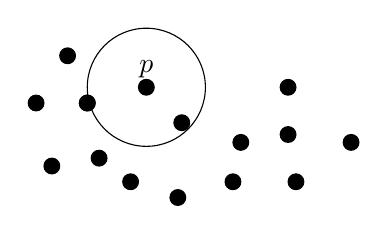
\begin{tikzpicture}


\draw[black, fill = black] (5,2) circle(0.1cm);
\draw[black](5,2)circle(0.75cm); 
\draw[anchor = south](5,2) node {$p$};  

\draw[black, fill = black] (5.45,1.55) circle(0.1cm);
\draw[black, fill = black] (4.25,1.8) circle(0.1cm);
\draw[black, fill = black] (4.25,1.8) circle(0.1cm);
\draw[black, fill = black] (4.0,2.4) circle(0.1cm);
\draw[black, fill = black] (3.6,1.8) circle(0.1cm);
\draw[black, fill = black] (3.8,1) circle(0.1cm);
\draw[black, fill = black] (4.4,1.1) circle(0.1cm);
\draw[black, fill = black] (4.8,0.8) circle(0.1cm);
\draw[black, fill = black] (5.4,0.6) circle(0.1cm);
\draw[black, fill = black] (6.1,0.8) circle(0.1cm);
\draw[black, fill = black] (6.2,1.3) circle(0.1cm);
\draw[black, fill = black] (6.8,1.4) circle(0.1cm);
\draw[black, fill = black] (6.9,0.8) circle(0.1cm);
\draw[black, fill = black] (6.8,2) circle(0.1cm);
\draw[black, fill = black] (7.6,1.3) circle(0.1cm);

\end{tikzpicture}
	\caption{Density-reachable example}
	\label{fig:density}
\end{figure} 

Finally, an object $p$ is density connected to an object $q$ if there exist an object $o$ such that both $p$ and $q$ are density-reachable from $o$, such as shown in \cref{fig:densityconn}.Note that all these properties are dependent on $\varepsilon$ and $MinPts$. In literature, for instance, it would be said that an object is density connected to another object with respect to $\varepsilon$ and $MinPts$, however this statement has been omitted since it is implied. 
\begin{figure}[h!]
	\centering
	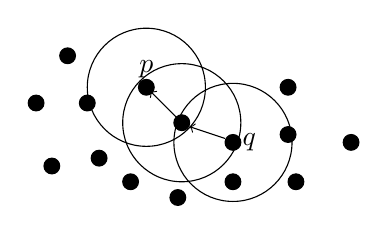
\begin{tikzpicture}


\draw[black, fill = black] (5,2) circle(0.1cm);
\draw[black](5,2)circle(0.75cm); 
\draw[anchor = south](5,2) node {$p$};  

\draw[black, fill = black] (5.45,1.55) circle(0.1cm);
\draw[black](5.45,1.55)circle(0.75cm); 


\draw[black, fill = black] (6.1,1.3) circle(0.1cm);
\draw[black](6.1,1.3)circle(0.75cm); 
\draw[anchor = west](6.1,1.3) node {$q$};  

\draw[black, fill = black] (4.25,1.8) circle(0.1cm);
\draw[black, fill = black] (4.0,2.4) circle(0.1cm);
\draw[black, fill = black] (3.6,1.8) circle(0.1cm);
\draw[black, fill = black] (3.8,1) circle(0.1cm);
\draw[black, fill = black] (4.4,1.1) circle(0.1cm);
\draw[black, fill = black] (4.8,0.8) circle(0.1cm);
\draw[black, fill = black] (5.4,0.6) circle(0.1cm);
\draw[black, fill = black] (6.1,0.8) circle(0.1cm);
\draw[black, fill = black] (6.8,1.4) circle(0.1cm);
\draw[black, fill = black] (6.9,0.8) circle(0.1cm);
\draw[black, fill = black] (6.8,2) circle(0.1cm);
\draw[black, fill = black] (7.6,1.3) circle(0.1cm);


\draw[->] (6,1.35)--(5.55,1.5); 
\draw[->] (5.4,1.6)--(5.05,1.95); 

\end{tikzpicture}
	\caption{Density-reachable example}
	\label{fig:densityconn}
\end{figure} 

With the previous definitions, one can now define the concepts of a \textit{density-conenected set}, which is a subset $C$ of a database $D$ that satisfies the following conditions 
\begin{enumerate}
	\item Maximality: For all $p$,$q \in D$: if $p \in C$ and $q$ is density-reachable from $p$, then $q\in C$.
	\item Connectivity: For all $p$,$q\in C$: $p$ is density-connected to $q$. 
\end{enumerate}

Now, one can define how a database should be decomposed after the clustering algorithms have been applied. The result is called \ac{dbd} and should meet the following conditions 

\begin{enumerate}
	\item $DBD = \{S_1,...,S_.,N\},k \geq 0$
	\item $S_1\cup ... \cup S_k \cup = D$
	\item For all $i \leq k$: $S_i$ is a \textit{density-connected} set
	\item  If there exists a \textit{density-connected} set $S\in D$, then there exists an $i \leq k$ so that $S =S_i$ 
	\item $N = D\setminus (S_1\cup...\cup S_k) $ is called the noise with respect to the decomposition $DBD$.
\end{enumerate}

This decomposition should be the output of the clustering algorithms where the subsets $S_i$ are the clusters and $N$ are any detections that were not assigned to any cluster. 